\section{System Development Methodology}

This study employs a structured system development methodology following the Agile approach. Agile was chosen for its flexibility and iterative nature, which allows for continuous refinement and adaptation of the system based on feedback and testing results. Each development phase—planning, design, implementation, testing, and deployment—will include regular reviews and adjustments to ensure the system evolves effectively to meet technical and user needs.
The system development process is divided into several distinct phases, each of which is designed to build upon the previous stage, ensuring a comprehensive and systematic approach.
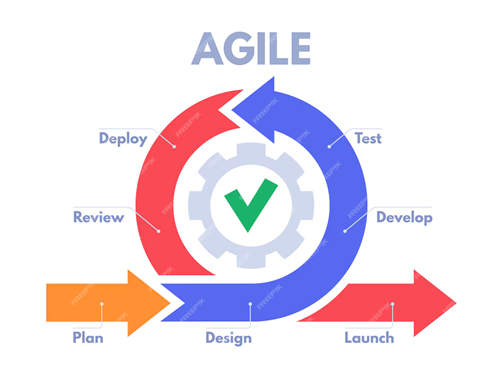
\includegraphics{AGILE}

\subsection{Planning}

In the initial phase, the researchers outlined the shelter location allocation system's scope, objectives, and requirements. This process identifies the key features and functionalities essential for the system. Additionally, this phase includes the thesis project plan, which details the project timeline.
The Gantt chart outlines the phases of the thesis project, including thesis one output, thesis two output, data collection and preparation, paper miscellaneous, system design, system development, and system assessment. Each phase addresses specific objectives that contribute to completing the shelter location-allocation system.
\textbf{Thesis One Output:} This phase involves drafting the initial sections of the thesis, such as the overview, rationale, scope, and significance, along with Chapters one through three (Introduction, Review of Related Literature, and Methodology). Additionally, this phase includes preparing the proposal manuscript, slides, and script for the mock defense and proposal defense. Parallel to this is the Paper Miscellaneous, which includes the creation of the literature review matrix to organize and support the contents of Chapter 2. This approach maintains a well-structured reference base for literature review.
\textbf{Thesis Two Output:} Following the foundational work in the first thesis phase, this continues the development of this thesis document, focusing on Chapters 4 and 5 (Results and Conclusions) and preparing for the mock defense and final thesis defense. This phase signifies the completion of the thesis writing process.
\textbf{Data Collection and Preparation:} This critical phase entails gathering data required for system design and important data for the genetic algorithm. Tasks include submitting documents to the LGU, presenting the project proposal, conducting client interviews, and collecting online and onsite data.
\textbf{System Design:} This phase focuses on planning the technical aspects of the shelter allocation system, including genetic algorithm implementation, user interface design, entity relationship diagram, and flowchart development. These elements form the blueprint that guides the system's development.
\textbf{System Development:} The project's core phase involves the actual construction and coding of the system. Tasks include front-end development, data integration, model integration, dashboard creation, and implementing security features. This phase also includes testing and debugging to ensure system functionality.
\textbf{System Assessment:} The final phase, along with Thesis Two Output, is evaluating the system's acceptability and user satisfaction. Activities include preparing and distributing surveys, gathering user feedback, and encoding and analyzing this data to assess system performance.

\subsection{Requirement Analysis}

During the requirement analysis phase, researchers gather comprehensive information about the system requirements by reviewing relevant literature that pertains to the thesis. This phase ensures that all necessary features are identified and prioritized based on their importance.
The system's primary features and requirements encompass an overview of data modification, data simulation, shelter tagging, and system security. Data modification includes an admin role responsible for managing community and shelter data, which can modify shelter and community data; data simulation utilizes the community and shelter data as inputs for the genetic algorithm applied in the shelter location allocation system, optimizing the placement of evacuees in shelters. Furthermore, shelter tagging enables the categorization of shelters based on criteria such as location, capacity, and suitability for various disaster scenarios, thereby facilitating efficient resource allocation. Lastly, system security ensures data protection and controlled access to maintain the integrity and confidentiality of the information managed by the system.

\subsection{Design}

During the design phase, the researchers created a detailed design outlining the shelter location-allocation system's architecture and key components. The design process includes creating a mockup of the system's user interface and constructing flowcharts, an entity-relationship diagram (ERD), and a context diagram to map out system processes and data relationships. The researchers designed mockups to visualize the user interface, ensuring it met the user's needs for accessibility and usability. The flowcharts provided a step-by-step breakdown of system processes, while the ERD defined the data structures and relationships. These elements formed a cohesive blueprint to guide the system's development and ensure alignment with the system's requirements. 
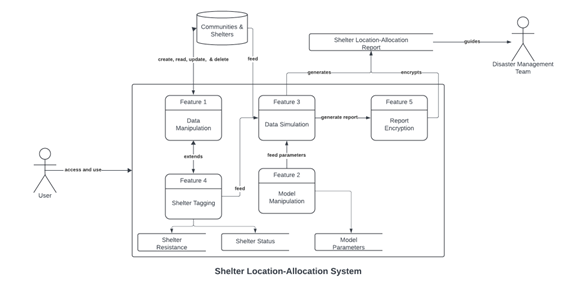
\includegraphics{DESIGN}
The system architecture involves the interaction of two actors, the user of the system and the disaster management team. The community and shelter data will be fed into a system which features data manipulation and shelter tagging. With the cleaned or finished data, data simulation may begin together with the model parameters modified by the user. Finally, a report will be generated and can be encrypted or not. The report will be used by the disaster management team to guide them for decision making in allocation of residents to the correct shelter.
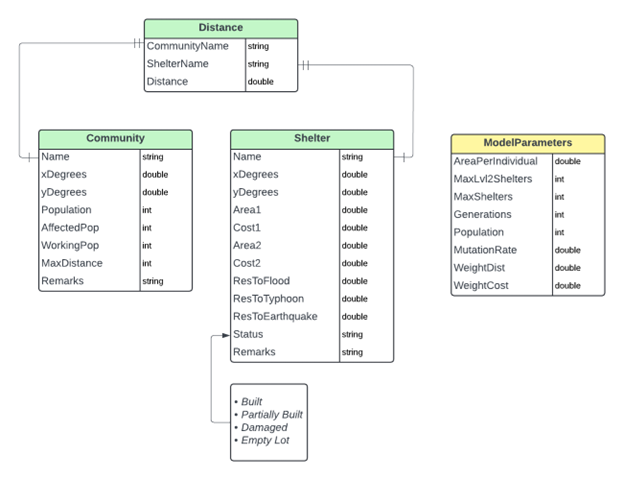
\includegraphics{ERD}
This diagram shows the entity relationship (ERD) which has 4 entities: Community, Shelter, Distance, and ModelParameters. Distances are derived from the location of Shelter and Community and will be saved accordingly to be used in performing the system model. ModelParameters shows no relationship since it only saves the current settings for the model and algorithm.
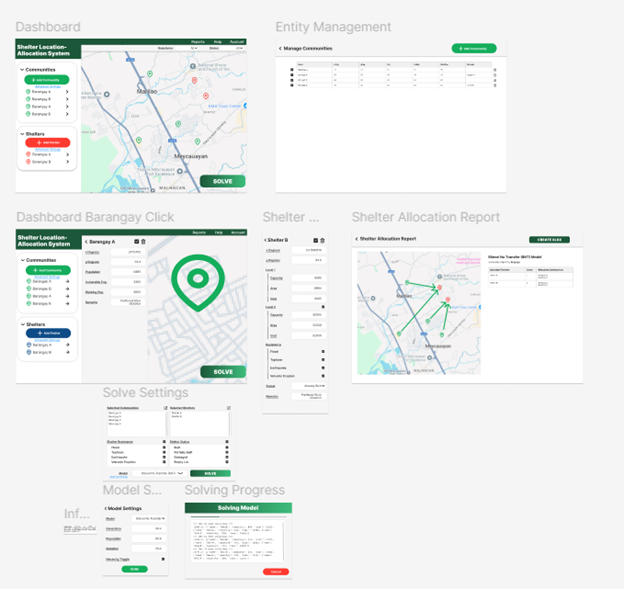
\includegraphics{SYSTEM MOCKUP}
The system mock-up shows the prototype of the system by designing the User Interface (UI) using a prototyping tool, Figma. This shows the UI for the different modules of the system: Dashboard, Entity Management, Shelter Allocation Report, Settings, and the Progress.

\textbf{Development}
The development phase will include coding and implementing the genetic algorithm for the shelter location allocation system. Utilizing the Agile system development life cycle, which includes weekly meetings and development reviews, the team can ensure that development remains on track and that any issues are promptly addressed. By following the Agile SDLC, the researchers can adapt quickly to any changes in requirements, maintain clear communication, and address any issues promptly.

\textbf{Testing}
The system will undergo functionality, performance, and reliability testing during the testing phase. The researchers will employ manual testing techniques to identify and resolve any bugs or issues that arise. This phase will also evaluate the system against the ISO/IEC 25010 standard to ensure its usability, reliability, and overall quality. Through this thorough testing approach, the researchers aim to ensure that the shelter location allocation system meets high quality, performance, and user satisfaction standards, making it ready for deployment.
\textbf{Development}
During the deployment phase, the shelter location-allocation system will undergo pilot testing in collaboration with local government units (LGUs). This process will involve configuring the system, establishing the necessary data inputs, and training users to utilize the platform effectively. Additionally, the deployment phase will continuously monitor the system's performance to ensure it operates efficiently and meets the objective of optimizing shelter locations. 
\textbf{Maintenance}
The maintenance phase will thoroughly identify and resolve any issues or bugs that may arise during regular operations. Maintenance involves actively monitoring the system's performance and user feedback to ensure a swift response to any problems encountered. Additionally, the researchers will prioritize implementing new features and enhancements based on valuable user feedback, ensuring the system evolves to meet user needs effectively.
\textbf{System Evaluation}
This section will focus on assessing the acceptability of the shelter location allocation system using the ISO/IEC 25010 standard. This standard provides a framework for evaluating the software's quality, usability, reliability, and performance efficiency. The system evaluation will include the evaluation instrument, determining the population and sample, outlining data collection procedures, and discussing the data analysis techniques used.
